\label{chapter:ModelBuild}
The first step in any model build is to develop a conceptual model, which defines the extent, inflows and outflows, material distributions and physical properties of a hydrogeologic flow system, real or imaginary. The intent of \mut\ is to then facilitate the production of a set of \mfus\ input files by minimizing the amount of time we spend building and testing it.  This chapter describes our current model build workflow, which can provide a sound basis for developing your own personal workflow.

The steps in our model build workflow are:
\begin{enumerate}
    \item Create a new working folder or copy an existing \mut\ project folder. \label{step:copy}
    \item Modify the \mut\ input file (and other input files if necessary) to reflect the new Modflow project.\label{step:modify}
    \item Run \mut\ to build the new Modflow project, which also produces \tecplot\ output files for the various Modflow domains (i.e. \gwf, \swf\ and/or \cln ) created during the build process. \label{step:mut1}
    \item Run \tecplot\ and examine the build output files.   \label{step:Tecplot1}
    \item Repeat steps~\ref{step:modify}-\ref{step:Tecplot1} until the new project is defined to your satisfaction.
\end{enumerate}

A \mut\ input file is a plain ascii text file that you can edit with your preferred editor (e.g. Windows Notepad\footnote{Our personal favourite editor is WinEdt (\url{https://www.winedt.com/snap.html}), which also provides a nice \LaTeX\ document development environment when coupled with the \TeX\ software package MiKTeX.  This manual was produced using these word processing tools.}).
The \mut\ input file name can have a prefix of your choice, followed by the extension \texttt{.mut}. Examples of valid \mut\ input file names are \texttt{\_build.mut} or \texttt{good.mut}. Most often, the easiest approach is to copy an existing input file and modify it as required.  This helps reduce set-up time and avoid potential errors that are introduced when creating input files from scratch.

To illustrate our model build workflow, we will refer to the various conceptual models developed for our existing suite of examples described in  Chapter~\ref{chapter:ModelVerification}.  As you read along, we urge you to carry out the steps we describe as we move through the workflow.  We recommend copying the contents of an existing model to a new location (e.g.\ copy the folder \texttt{1\_VSF\_Column} to \texttt{C:$\backslash$SandBox}).
\pagebreak 
If you did so, your working directory would look something like this:

    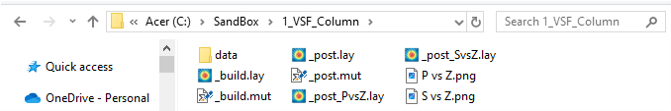
\includegraphics[width=\textwidth]{3_1_vsf_column_folderinit}

In the \texttt{1\_VSF\_Column} example, there is a \mut\ input file for the model build called \texttt{\_build.mut} and a \tecplot\ layout file called \texttt{\_build.lay} used to visualize the model build results.  The rest of the files are related to post-processing \mfus\ model results and will be discussed later in chapter~\ref{chapter:ModelExecution}.
 
 In our preferred workflow we would first start a command prompt in the folder which contains the \mut\ input file by:
\begin{enumerate}
   \item  Navigating to the folder in File Explorer (e.g.\ \texttt{C:$\backslash$SandBox$\backslash$1\_VSF\_Column}).
   \item  Highlighting the path in File Explorer:

        
\includegraphics[width=0.3\textwidth]{3_3_HighlightPath}

    \item  Replacing the existing path with the string {\sf cmd}:

        
\includegraphics[width=0.5\textwidth]{3_4_cmd}

    \item Pressing Enter/Return.
\end{enumerate}
A command prompt window rooted at the input folder should appear:

        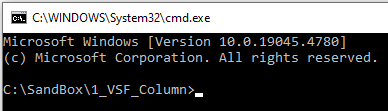
\includegraphics[width=0.4\textwidth]{3_5_cmdPrompt}



When you run \mut\, it will try to obtain a prefix in the following order:
\begin{enumerate}
    \item \textbf{From a command line argument:} \label{commarg} At the command prompt, \mut\ checks for the presence of a command line argument.  For example, typing this:
\begin{verbatim}
    mut Good
\end{verbatim}
        would cause \mut\ to process the input file \texttt{Good.mut}.
    \item \textbf{From a prefix file:} If there is no command line argument, \mut\ checks for the presence of the file \texttt{\_mut.pfx} in the folder.  If present, \mut\ will read the prefix from it. For example, if the mut file was called \texttt{Good.mut} then the file \texttt{mut.pfx} would contain the single line:
\begin{verbatim}
    good
\end{verbatim}
    \item \textbf{From the default input file:} If there is no command line argument or prefix file in the folder, \mut\ checks for the presence of the file \texttt{a.mut}.  If present in the folder, \mut\ will process it.
    \item \textbf{From the keyboard:} If none of these methods are successful, \mut\ will prompt for a prefix as shown here:

        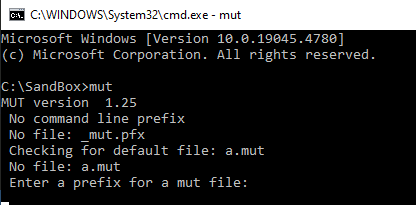
\includegraphics[width=0.6\textwidth]{3_2_mut_no_prefix}

        The user would type the prefix e.g.: \texttt{good} and press Enter.

\end{enumerate}

To build the \texttt{1\_VSF\_Column} example, we would  run \mut\ using the input file \texttt{\_build.mut} by typing:
\begin{verbatim}
    mut _build
\end{verbatim}
which uses the first method to supply the prefix.


If you open the file \texttt{\_build.mut} in a text editor you will see the first couple of lines are comments (which begin with an exclamation point character: '{\tt !}') describing the problem:
\squish
\begin{verbatim}
    ! Examples\1_VSF_Column:
    !   A modflow project of a 1D column generated from a simple 2d rectangular mesh
\end{verbatim}
 \mut\ first creates a clean copy of the input file called \texttt{\_buildo.input} by removing all comment lines.

 As \mut\ processes the input file, output is written to both the screen and to the file \texttt{\_buildo.eco}.  If you open \texttt{\_buildo.eco}, you will see the first thing written is the \mut\ header, which contains the version number and build date.

 These are followed by the stripped comments, which  can provide a synopsis of the input file contents. The rest of the cleaned input file contains \mut\ instructions, which may require data in the form of numbers (e.g.\ parameter values) or alphanumeric strings (e.g.\ file names).


The first instruction in the cleaned input file begins the model build:

\ins{build modflow usg}
    {This  is a {\em subtask} that defines the characteristics of the \mfus\ model including:
     \begin{itemize}
        \item Units of length and time.
        \item Numerical model meshes.
        \item Material properties.
        \item Boundary conditions.
        \item Time-stepping, stress period and output control parameters.
        \item Solver parameters.
    \end{itemize}

    An end instruction is required to stop the subtask e.g.:

    {\Large \sf end build modflow usg}
    }

After \mut\ finishes, the working folder should look something like this:

        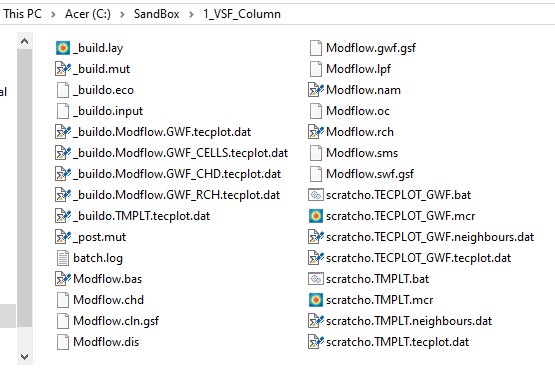
\includegraphics[width=0.8\textwidth]{3_6_buildFiles}

Several new output files have been created, of which it may be noted:
\begin{itemize}
    \item Build output files, which have the prefix \texttt{\_buildo}, appear near the start of the list if sorted by name. \mut\ deletes previously generated build output files and writes a fresh set each time it is run.  This can prevent confusion that might arise if out-of-date output files were present.\footnote{For example, if we define a recharge boundary condition, \mut\ will create the file \texttt{\textit{prefix}o.Modflow.SWF\_RCH.Tecplot.dat} which shows the locations and recharge values assigned to Modflow cells.  If we then removed the recharge condition from the input file, but did not delete this output file, we may assume the recharge condition still applies.}
    \item \tecplot\ output files are indicated by the suffix \texttt{.tecplot.dat}.
    \item Modflow model input files are written using the default prefix \texttt{Modflow}, (e.g.\ \texttt{Modflow.nam, Modflow.bas} etc.)  The prefix can be customized if desired but there are advantages to keeping this 'generic' one, such as portability of post-processing scripts or \tecplot\ layout files that follow this generic naming convention.
    \item Several scratch files (with prefix \texttt{scratcho}) are written. These are used for debugging during code development and can be ignored in most cases.
    \item If the run is successful the last line written will be \texttt{Normal exit}, otherwise an error message will be given.
\end{itemize}

